% Dokumentanklasse: a4paper, 14pt
% Beschreibung:     Dokumentenformat
% Option:           extraarticle - ?
\documentclass[a4paper,14 pt]{extarticle}

% Paket:            a4paper
% Beschreibung:     A4 Seitenabstände
% Option:           geometry
\usepackage{geometry}
\geometry{
	paper=a4paper, 	% Papierformat
	%top=3cm, 		% Kopf-Spannweite
	%bottom=1.5cm,	% Fuß-Spannweite
	%left=4.5cm, 	% Linke-Spannweite
	%right=4.5cm,	% Rechte-Spannweite
	%showframe,		% Uncomment to show how the type block is set on the page
}

% Paket:            ansmath
% Beschreibung:     Zum darstellen von mathematischen Formeln
\usepackage{amsmath}

% Paket:            ngerman
% Beschreibung:     Deutsche Rechtschreibung
% Option:           babel - Sibentrennung
%\usepackage{ngerman}
\usepackage[ngerman]{babel}

% Paket:            utf8
% Beschreibung:     Stellt Umlaute richtig dar
% Option:           inputenc - Erlaubt die Darstellung der gleichen Zeichen (Character) wie sie in strin überliefert werden
\usepackage[utf8]{inputenc}

% Paket:            makeindex
% Beschreibung:     Ermöglicht das Indexieren von Wörter und den Befehl \printindex um den Index auszugeben
\usepackage{makeidx}
\makeindex

% Paket:            natbib
% Beschreibung:     Für Zitate
% Option:           round - ?
%\usepackage[round]{natbib}

% Paket:            fancyhdr
% Beschreibung:     Ermöglich ein generelles Seitenlayout ein zu stellen mit Kopf und Fußzeile.
\usepackage{fancyhdr}

% Paket:            graphicx
% Beschreibung:     Einbinden von Bildern
% Option:
\usepackage{graphicx}

% Paket:            enumitem
% Beschreibung:     Zeilenabstände bei Aufzählungen definieren
% Option:
\usepackage{enumitem}

% Paket:            float
% Beschreibung:     Zum Ausrichten von Tabellen und Spalten bzw deren zentrierung
% Option:
% Restriktion:      Muss von Paket hyperref geladen werden. Ansonsten funktioniert das Paket nicht.
\usepackage{float}

% Paket:            appendix
% Beschreibung:     Das Paket dient dazu, ausschließlich das Thema einer Überschrift in das Inhaltsverzeichnis zu überführen
% Option:           appendix - Überführt die Überschriften des Anhangs richtig ins das Inhaltsverzeichnis
\usepackage[titletoc]{appendix}

% Paket:            setspace
% Beschreibung:     Setz über die optionen den Zeilenabstand
% Optionen:         Möglicher Zeilenabstand
%                   singlespacing = 1,0
%                   onehalfspacing = 1,5
%                   doublespacing = 2,0
% Restriktion:      Muss von Paket hyperref geladen werden. Ansonsten funktioniert das Paket nicht.
\usepackage[onehalfspacing]{setspace}

% Packet:           Hyperref
% Beschreibung:     Importiert hyperref um Querverweise mittels \hyperref zu erzeugen.
\usepackage[]{hyperref}
\hypersetup{
  pdftitle={PDF-Title},
  pdfauthor={Markus Pesch},
  pdfsubject={PDF-Subject}
}

% Packet:           Minted
% Beschreibung:     Dient zum highlining von Quellcode wie beispielsweise Java, Bash oder Python.
\usepackage{minted}
\usemintedstyle{emacs}

% Packet:           tabularx
% Beschreibung:     Werden Tabellen mit diesem Paket erstellt, ist es möglich Zeilenumbrüche in einer Zelle zu erzeugen
\usepackage{tabularx}


% Paket: biblatex
\usepackage[
  style=authoryear-icomp,  	% Zitierstil
  isbn=false,				% Die ISBN Nummer ausblenden				
  pagetracker=true,        	% ebd. bei wiederholten Angaben (false=ausgeschaltet, page=Seite, spread=Doppelseite, true=automatisch)
  maxbibnames=50,          	% maximale Namen, die im Literaturverzeichnis angezeigt werden (ich wollte alle)
  maxcitenames=3,          	% maximale Namen, die im Text angezeigt werden, ab 4 wird u.a. nach den ersten Autor angezeigt
  autocite=inline,         	% regelt Aussehen für \autocite (inline=\parancite)
  block=space,             	% kleiner horizontaler Platz zwischen den Feldern
  backref=true,            	% Seiten anzeigen, auf denen die Referenz vorkommt
  backrefstyle=three+,     	% fasst Seiten zusammen, z.B. S. 2f, 6ff, 7-10
  date=short,              	% Datumsformat
  backend=biber
]{biblatex}
\setlength{\bibitemsep}{1em}     % Abstand zwischen den Literaturangaben
\setlength{\bibhang}{2em}        % Einzug nach jeweils erster Zeile

\addbibresource{literatur//bibliothek.bib}


% Packet:           glossaries
% Beschreibung:     Glossar einbinden und Glossarbefehle bereitstellen
% Option:           Gebe Glossar auch als section im Inhaltsverzeichnis aus
\usepackage[toc,section=section]{glossaries}
\makeglossaries
\include{glossar//glossar}

% Paket:			xcolor
% Beschreibung:		Definition eigener Farben
\usepackage[usenames,dvipsnames]{xcolor}
\definecolor{orange}{HTML}{FF7F00}

% Einstellungen überschreiben
\newcommand{\myparagraph}[1]{\paragraph{#1}\mbox{}\\}

% Frame-Blöcke
\usepackage[framemethod=tikz]{mdframed}
\mdtheorem[
  linecolor=red,
  frametitlefont=\sffamily\bfseries\color{white},
  frametitlebackgroundcolor=red,
]{WARN}{Warnung}[subsection]

\mdtheorem[
linecolor=orange,
frametitlefont=\sffamily\bfseries\color{white},
frametitlebackgroundcolor=orange,
]{INFO}{Information}[subsection]

\usepackage{lscape}

% Start des Dokuments
\begin{document}

  % Fetch Commit ID and Date
  \immediate\write18{./git-info.sh commit > git-id.tmp}
  \immediate\write18{./git-info.sh date > git-date.tmp}
  \immediate\write18{./git-info.sh url > git-url.tmp}

  % Importiere weitere .tex Dokumente
  \begin{titlepage}
	\begin{center}
		
		\begin{huge}
			\begin{singlespace}
				\textbf{Seminar - Data Science}
			\end{singlespace}
		\end{huge}
		
		\vspace{1.2cm}
		
		\begin{Large}
			Das Revisionssystem git
		\end{Large}
		
		\vspace{0.5cm}
		
		\begin{figure}[h]
			\centering
			\includegraphics[width=0.85\textwidth]{images//logo.png}
			\label{img:fh-trier-logo}
		\end{figure}
		
		\vspace{1.5cm}
		
		\begin{large}
			Markus Pesch\\
			peschm@hochschule-trier.de
		\end{large}
		
		\vspace{2cm}
		
		Latex Quellcode auf \input{./git-url.tmp} \\
		basierend auf git commit \input{git-id.tmp} vom \input{git-date.tmp}
		
	\end{center}
\end{titlepage}

  \pagebreak

  % Pagestyle
  % Setze das Seitenlayout auf leer um Fuß und Kopfzeilen zu unterdrücken
  \pagestyle{empty}

  % Importiere weitere .tex Dokumente
  \section*{Vorwort}
Dieses Dokument soll den Leser den Umgang mit Git näher bringen. Dazu wird Ihm der Umgang mit den gängigen Git-Befehlen näher gebracht und der Workflow von üblichen Online-Repositories erläutert. 

Als Beispiel wird in diesem Dokument ein Workflow eingerichtet, die dem Entwickler ermöglicht Quellcodeverbesserungen an diesen Dokument durch Merge Requests vorzunehmen.

\newpage


  \include{agenda//agenda}

  % Pagestyle
  % Setze das Seitenlayout auf fancyhdr um Fuß- und Kopfzeilen zu setzen
  \pagestyle{fancy}

  % Löscht alle Kopf- und Fußzeilen des pagestyles fancyhdr
  \fancyhf{}

  % Fuß- und Kopfzeile des Paketes fancyhdr
  % [L] - Linkeseite      [O] - Ungerade Seitenzahlen         [LE,LO] - Linkeseite, Gerade- und Ungerade Seitenanzahlen
  % [C] - Mitte           [E] - Gerade Seitenanzahlen         [CE]    - Seitenmitte, nur gerade Seitenanzahlen
  % [R] - Rechteseite                                         [RO]    - Rechteseite, nur ungerade Seitenanzahlen
  % \fancyhead    Kopfzeile
  % \fancyfoot    Fußzeile
  \fancyhead[L]{\rightmark}
  \fancyhead[R]{Seite \thepage}

  % Pixelstärke der Kopfzeilenlinie
  \renewcommand{\headrulewidth}{1pt}

  % Setze die Seitenbeginn zurück
  \setcounter{page}{1}

  % Importiere weitere .tex Dokumente
  \label{sec:einfuehrung}
\section{Einführung}
Dieses Kapitel bietet eine Einführung in die Grundbegriffe von Git und deren Konfigurationseinstellungen. Fortlaufend wird auf Basis dieses \LaTeX{} Dokuments gezeigt, wie ein Projekt mit Git unter Versionskontrolle gestellt werden kann. Dazu werden die wichtigsten Git-Kommandos näher erläutert.

\label{sec:einfuehrung.grundbegriffe}
\subsection{Grundbegriffe}
Um dem Umgang mit Git zu erläutern ist es notwendig, einige Fachbegriffe zu verstehen. 

\myparagraph{Versionskontrollsystem} 
Ein Versionskontrollsystem dient zur Verwaltung und Versionierung von Software. Bekannte Projekte die unter dem Versionskontrollsystem Git stehen sind beispielsweise der Linux-Kernel und Git selbst. Beide Projekte stehen unter der Lizenz GPL. Der Quellcode kann mittels git bezogen werden. Dazu später mehr.

Bei Versionskontrollsystemen wird unterschieden zwischen zentralen und dezentralen Systemen. Git ist ein dezentrales System. Der Entwickler ist nicht abhängig von dem Server auf dem die Versionshierarchie gespeichert ist. Der Entwickler ist in der Lage mit Git die komplette Versionshierarchie auf sein eigenes System zu klonen und auf dieser Basis zu arbeiten.   

\myparagraph{Repository}
Git  verwaltet von jeder Datei unterschiedliche Zustände bzw. Versionen. Diese werden in dem Repository gespeichert. Mithilfe des Repositories ist es möglich, auf jeden Zustand einer Datei zurück zu springen.

\myparagraph{Working Tree}
Alle Modifikationen an Dateien bzw. dem Quellcode werden im Working Tree vorgenommen. Andere Bezeichnungen hierfür sind auch Working Directory oder Workspace. Wobei bei vielen IDEs im Heimatverzeichnis das Verzeichnis workspace erstellt wird um Projekte zu speichern und unter Versionskontrolle zu setzen. 

\myparagraph{Commit}
Ein Commit nimmt jede Veränderung, Modifikation oder Erstellung an Dateien im Working Tree auf. Zusätzlich speichert der Commit noch weitere Informationen wie den Benutzernamen und dessen E-Mail mit Datum und optional gpg-Signatur ab.  

\myparagraph{HEAD}
HEAD bildet eine Referenz ab, in welchem Zustand der Entwickler sein Working Tree vor findet. 

\myparagraph{Branch}
Jede Software kann in ihrem Verlauf mehrere Entwicklungsverzweigungen haben um beispielsweise in jeder Verzweigung einzelne Teilaufgaben wie Patches oder neuen Features von Software zu entwickeln. Diese Verzweigungen werden Branches genannt. Jede Verzweigung kann später durch einen Merge oder Rebase wieder zurück geführt werden.


\label{sec:einfuehrung.git}
\subsection{Einrichtung von Git}
Wie bereits in in Kapitel \ref{sec:einfuehrung.grundbegriffe} erklärt, speichert Git bei jedem Commit den Benutzernamen und E-Mail ab. Bevor nun dieses Dokument, das als \LaTeX{} Projekt angelegt wurde, durch Git verwaltet wird, ist es Sinnvoll den Benutzernamen und die E-Mail Adresse anzupassen \footcite{git-1.6-your-identity}.

\begin{minted}[linenos, framesep=2mm, fontsize=\small]{bash}
$ git config --global user.name "Hugo McKinnock"
$ git config --global user.email "hugo.mckinnock@example.com"
\end{minted}

Ist ein gpg Schlüssel vorhanden, kann dieser direkt hinterlegt werden um Commits direkt im Hintergrund zu signieren. Dazu muss zuerst der gpg Schlüssel ausfindig gemacht werden und anschließend Git mitgeteilt werden.

\begin{minted}[linenos, framesep=2mm, fontsize=\small]{bash}
$ gpg --list-secret-keys --keyid-format 0xSHORT
/home/hugo/.config/gnupg/pubring.gpg
--------------------------------------
sec   rsa4096/0x85ED78DE 2018-03-15 [SC] [verfällt: 2018-09-15]
uid        [  ultimativ] Hugo McKinnock <hugo.mckinnock@example.com>
ssb   rsa4096/0x848DEAC1 2018-03-15 [E] [verfällt: 2018-09-15]

$ git config --global user.signingkey "0x85ED78DE"
$ git config --global commit.gpgSign true
\end{minted}

\section{Projekt auschecken}
Wir erstellen im Heimatverzeichnis, wie von den meisten IDE's bevorzugt, das Verzeichnis \textit{workspace} und klonen von einem Online-Repository dieses Projekt. Anschließend befindet sich im Verzeichnis \textit{workspace} der Unterordner \textit{sdsm\_ss17\_git} in den wir navigieren. 

\begin{minted}[linenos, framesep=2mm, fontsize=\small]{bash}
$ mkdir ~/workspace
$ git clone https://git.cryptic.systems/fh-trier/sdsm_ss17_git.git
$ cd sdsm_ss17_git
\end{minted}

\begin{INFO}
  Zum klonen eines Online-Repositories wird auf vielen Online-Plattformen wie \href{https://github.com}{GitHub} oder \href{https://gitlab.com}{GitLab} eine Adresse per \textit{HTTPS-} oder \textit{SSH-}Protokoll angeboten. 
  
  Für eine Verbindung per SSH-Protokoll muss ein Account auf diesen Online-Plattformen registriert sein und der öffentliche Schlüssel des asymmetrischen Verschlüsselungsverfahren hinterlegt sein.  
\end{INFO}

Das heruntergeladene Repository spiegelt nun den Zustand ab, auf dem sich die Referenz \textit{HEAD} befindet. Um dies zu überprüfen, bietet Git den Befehl \textit{git log} an. Wir lassen uns die neusten zwei Commits anzeigen.

\begin{minted}[linenos, framesep=2mm, fontsize=\small]{bash}
$ git log -2
commit 4660915d6c031598c77b49c6275e426f7c3a85c3 (HEAD -> master, 
origin/master, origin/HEAD)
Author: Markus Pesch <markus.pesch@cryptic.systems>
Date:   Thu Mar 15 16:49:12 2018 +0100

add: chapter 1

commit 1ca84c7271f3f3c306b779256bd1902497f44fb9
Author: Markus Pesch <markus.pesch@cryptic.systems>
Date:   Thu Mar 15 13:26:02 2018 +0100

fix: geometry
\end{minted}

Zu erkennen ist, dass sich die Referenz \textit{HEAD} auf der gleichen Position wie der Branch \textit{master} befindet. Der Branch \textit{master} ist ein Branch auf dem lokalen System des Entwicklers. Die Referenz \textit{origin/master} zeigt den Zustand an, auf dem das Online-Repository, von dem geklont wurde, steht.

  \section{Workflow}
\label{sec:workflow}

\subsection{Erläuterung}
\label{sec:workflow.erlaeuterung}
Wie bereits in Kapitel \ref*{sec:einfuehrung.grundbegriffe} erwähnt, ist ein dezentrales Versionskontrollsystem. Dadurch ist jeder Nutzer in der Lage ohne Abhängigkeit zu einem Server seinen Quellcode zu versionieren.

Jeder Nutzer kann sein eigenes Projekt durch \textit{git init} zu einem Git Repository initialisieren oder ein bestehendes Repository aus einem Online-Verzeichnis klonen. Beim klonen des Repositories wird der komplette Hierarchiebaum bzw. die Chronik mit jedem Commit und Branch geklont. Beim initialisieren eines neuen Repositories ist der Hierarchiebaum leer und unbeschrieben. Die Initialisierung eines neues Repositories wird bevorzugt beim neuen Projekten.

Um jedoch einen Workflow einzurichten, der es ermöglicht an bestehenden Projekten teil zu nehmen, muss zuerst das Projekt auf das lokale System geklont werden. Nachdem das Projekt als Git Repository auf dem lokalen System vorhanden ist, können Änderungen am Quellcode vorgenommen werden und in den Hierarchiebaum bzw. dem Repository hinzugefügt werden. Ist der Entwickler der Meinung, das alle Änderungen abgeschlossen sind, obliegt ihm selbst ob er seine Änderungen an den Hauptverantwortlichen einreicht. 

Der Entwickler kann seine Änderungen als Patch per E-Mail einreichen, sofern die Hauptverantwortlichen des geklonten Projekts dieses Verfahren unterstützen. Die bevorzugte Methode ist bei den meisten Online-Plattformen jedoch der Merge Request, manchmal auch Pull-Request genannt. 

Bei einem Merge-Request fragt man an, ob eine bestimmte Sammlung von Commits, die eine Änderung des Quellcodes wieder spiegeln, durch die Hauptverantwortlichen übernommen werden. Dadurch wird der Hierarchiebaum des Online-Repositories um die eigenen Commits erweitert. Anderen Entwickler, die auch dieses Repository geklont haben, können zukünftig die Änderung aus dem Online-Repository auf ihr eigenes lokales Repository übernehmen.

\begin{figure}[h]
  \centering
  \label{img:workflow}
  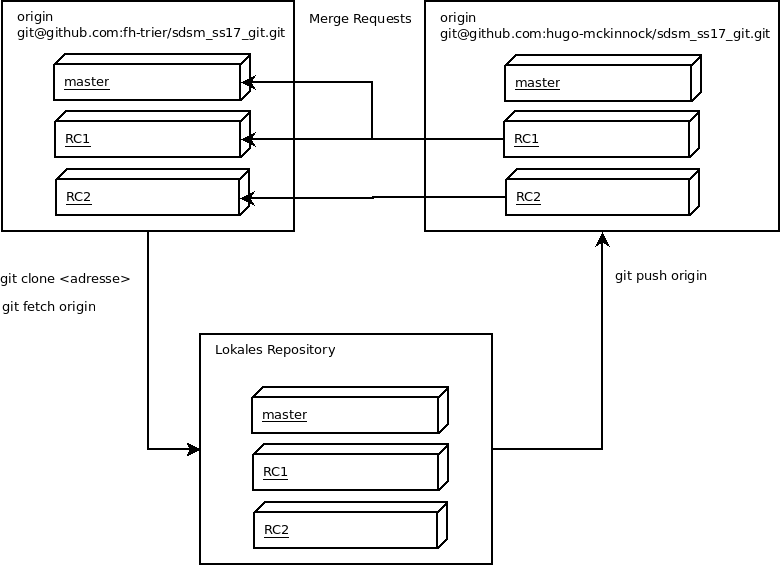
\includegraphics[width=1\textwidth]{images//workflow.png}
  \caption{Workflow}
\end{figure}  


\subsection{Einrichtung}
\label{sec:workflow.einrichtung}
Im Heimatverzeichnis wird wie von vielen IDE's bevorzugt, das Verzeichnis \textit{workspace} erstellt. Dort wird von dem Online-Repository \href{https://github.com}{GitHub} dieses \LaTeX{} Projekt, das dieses Dokument enthält, geklont. Nach dem klonen befindet sich im Verzeichnis \textit{workspace} der Unterordner \textit{sdsm\_ss17\_git}, in den mittels \textit{cd} nachträglich navigiert wird.

\begin{minted}[framesep=2mm, fontsize=\small]{bash}
$ mkdir ~/workspace
$ git clone git@github.com:fh-trier/sdsm_ss17_git.git
$ cd sdsm_ss17_git
\end{minted}

\begin{INFO}
  Zum klonen eines Online-Repositories wird auf vielen Online-Plattformen wie \href{https://github.com}{GitHub} oder \href{https://gitlab.com}{GitLab} eine Adresse per \textit{HTTPS-} oder \textit{SSH-}Protokoll angeboten. 
  
  Für eine Verbindung per SSH-Protokoll muss ein Account auf diesen Online-Plattformen registriert und der öffentliche Schlüssel des asymmetrischen Verschlüsselungsverfahren hinterlegt sein.  
\end{INFO}

Das heruntergeladene Repository spiegelt nun den Zustand wieder, auf dem sich die Referenz \textit{HEAD} befindet. Um dies zu überprüfen, bietet Git den Befehl \textit{git log} an. Wir lassen uns die neusten zwei Commits anzeigen.

\begin{minted}[framesep=2mm, fontsize=\small]{bash}
$ git log -2
commit e42f6e04ac8c3d2cf7d1e2c3b5dd5f7257612dc5 (HEAD -> master, origin/master)
Author: Markus Pesch <markus.pesch@cryptic.systems>
Date:   Thu Mar 15 21:59:24 2018 +0100

fix: chapter 2.2

commit 800ac8b5930ebe0650b83471aee957fe2195de05
Author: Markus Pesch <markus.pesch@cryptic.systems>
Date:   Thu Mar 15 21:53:14 2018 +0100

fix: chapter 2.
\end{minted}

Zu erkennen ist, dass sich die Referenz \textit{HEAD} auf der gleichen Position wie der Branch \textit{master} befindet. Der Branch \textit{master} ist ein Branch auf dem lokalen System des Entwicklers. Die Referenz \textit{origin/master} referenziert auf den Commit, auf dem das Online-Repository \textit{origin} und dessen Branch \textit{master} steht. Alle Referenzen referenzieren auf den Commit mit der ID \textit{e42f6e0}.

\begin{WARN}
  Zeigt \textit{HEAD} nicht auf einen Branch, spricht man davon, dass \textit{HEAD} losgelöst von einem Branch ist. Dies ist nur Sinnvoll um ältere Zustände zu betrachten, da auf einem losgelösten Zustand keine Änderungen angewandt werden können.
\end{WARN}

Um zu überprüfen welche Adresse sich hinter dem Label \textit{origin} befindet, bietet Git den Befehl \textit{git remote -v} an.

\begin{minted}[framesep=2mm, fontsize=\small]{bash}
$ git remote -v
origin  git@github.com:fh-trier/sdsm_ss17_git.git (fetch)
origin  git@github.com:fh-trier/sdsm_ss17_git.git (push)
\end{minted}

Zu erkennen ist, dass bei dem Befehl \textit{git fetch origin} alle neuen Commits von der Adresse \textit{git@github.com:fh-trier/sdsm\_ss17\_git.git} heruntergeladen werden - gekennzeichnet durch \textit{fetch}. Bei einem \textit{git push origin} versucht Git alle neuen Commits auf die gleiche Adresse, gekennzeichnet durch \textit{push}, zu schreiben. 

\begin{INFO}
  Lässt man das Label bei \textit{git fetch} und \textit{git push} weg, nimmt Git automatisch das Label \textit{origin} an. Das Label \textit{origin} ist das Standard-Label zur Bezeichnung von Remote-Adressen.
\end{INFO}

Möchte man nun seine Commits auf pushen, wird Git den push zurückweisen. Der Grund ist, dass man nicht der Eigentümer des Repositories unter der Adresse \textit{git@github.com:fh-trier/sdsm\_ss17\_git.git} ist. Um dies zu lösen, muss unter dem Label \textit{origin} die \textit{push}-Adresse geändert werden. Die einfachste Möglichkeit ist, sich auf der gleichen Online-Plattform, hier \href{https://github.com}{GitHub}, einen eigenen Benutzernamen zu registrieren und einen Ableger, auch Fork genannt, zu erzeugen. Man erhält anschließend eine neue Adresse, die den eigenen Benutzernamen enthält. 

Nun wird Git mitgeteilt, die neue Adresse als \textit{push}-Adresse unter dem Label \textit{origin} zu nutzen. Nach dem setzen werden die Adressen überprüft.

\begin{minted}[framesep=2mm, fontsize=\small]{bash}
$ git remote set-url origin \ 
      --add --push git@github.com:hugo-mckinnock/sdsm_ss17_git.git
$ git remote -v
origin	git@github.com:fh-trier/sdsm_ss17_git.git (fetch)
origin	git@github.com:hugo-mckinnock/sdsm_ss17_git.git (push)
\end{minted}

\begin{INFO}
  Möchte man sein Repository bei einem \textit{git push} Befehl auf mehrere Online-Repositories kopieren, dann kann der Befehl zum hinzufügen wiederholt werden unter Angabe einer weiteren Adresse.
\end{INFO}

Möchte man eine komplette Remote-Verbindung entfernen, kann dies unter Angabe des Git Befehls \textit{git remote remove  $ < $label $ > $} vorgenommen werden. 
  
Hinzufügen einer neuen Remote-Verbindungen ist möglich mit Angabe des neuen Labels mittels \textit{git remote add $ < $label$ > $ $ < $adresse$ > $}.

Nun ist der komplette Workflow eingerichtet und es wird Zeit sich mit den essentiellen Funktionen von Git zu beschäftigen. Dazu mehr in Kapitel 3.

  \section{Git-Befehle}
\label{git-commands}

Um am Workflow, wie er in Abbildung \ref{img:workflow} abgebildet ist teil zu nehmen, sind ein paar grundlegende Git-Befehle notwendig. Ein paar Befehle wurden bereits in Kapitel \ref{sec:einfuehrung.git} und \ref{workflow.einrichtung} vorgestellt.

\subsection{Weitere Git-Befehle}
\label{git-commands.advanced}

\myparagraph{git add}
\label{git-commands.advanced.add}
Der Befehl \textit{git add} fügt Veränderungen an einer Datei aus dem Working Tree dem Index hinzu. Wird eine Datei dem Index hinzugefügt, wird sie in dem Zustand dem Index hinzugefügt, wie sie sich zum Zeitpunkt beim ausführen des Befehls befindet. Dateien die sich im Index befinden sind für einen Commit vorgemerkt. 

\myparagraph{git commit}
\label{git-commands.advanced.commit}
Der Befehl \textit{git commit} speichert unter Angabe einer Nachricht den Zustand aller Dateien aus dem Index ab. Zusätzlich werden bei jedem Commit Metadaten mit abgespeichert wie bspw. der Name des Authors und dessen E-Mail Adresse. Optional kann dem Commit auch eine digitale Signatur hinzugefügt werden.

\myparagraph{git fetch}
\label{git-commands.advanced.fetch}
Mit \textit{git fetch $ < $label$ > $} werden alle neuen Commits von einem Online-Repository heruntergeladen, die sich noch nicht lokal auf dem System befinden.

\begin{INFO}
  Wenn der Befehl \textit{git fetch} ausgeführt wird, heißt dies noch nicht, dass das lokale Repository aktualisiert wird. Dies muss mittels \textit{\nameref{git-commands.advanced.merge}} oder \textit{\nameref{git-commands.advanced.rebase}} manuell ausgeführt werden.
\end{INFO}

\myparagraph{git push}
\label{git-commands.advanced.push}
Kopiert alle neuen Commits des aktuellen lokalen Branches auf einen Branch des Online-Repositories unter Angabe des Labels.

\myparagraph{git merge}
\label{git-commands.advanced.merge}
Fügt zwei Branches wieder zusammen. Beim Zusammenfügen können Konflikte entstehen, die der Entwickler manuell auflösen muss. Dazu bietet sich das Programm \textit{meld} an.

\myparagraph{git rebase}
\label{git-commands.advanced.rebase}
Schreibt die Historie bzw. Chronik eines Branches neu, in dem die neuen Commits auf \textit{HEAD} aufgesetzt werden. Bei einem \textit{rebase} kann es zu Konflikten kommen, die der Entwickler manuell auflösen muss. Dazu bietet sich das Programm \textit{meld} an. 

Der Vorteil gegenüber einem \textit{\nameref{git-commands.advanced.merge}} ist, dass wenn der Entwickler die Historie auflösen möchte, nicht alle Verzweigungen bzw Branches mit auflösen muss. Ein Rebase hält die Historie möglichst sauber.

\myparagraph{git reset}
\label{git-commands.advanced.reset}

\myparagraph{git revert}
\label{git-commands.advanced.revert}

\myparagraph{git log}
\label{git-commands.advanced.log}

\myparagraph{git status}
\label{git-commands.advanced.status}

\myparagraph{git diff}
\label{git-commands.advanced.diff}
  \section{Arbeiten mit Git}
\label{work-with-git}

\subsection{Erste Schritte}
\label{work-with-git.first-steps}
Nachdem wie in Abschnitt \ref{workflow.einrichtung} beschrieben die generelle Umgebung eingerichtet wurde, befindet sich im gleichen Verzeichnis die Datei \textit{test.sh}.

\begin{minted}[framesep=2mm, linenos, fontsize=\small]{bash}
#!/usr/bin/env bash
PWD="$(pwd)"
ls -la ${PWD} | grep -e '^d' 2>/dev/null
\end{minted}

\subsection{Modifikationen sichtbar machen}
\label{work-with-git.modifikation}
In der Datei \textit{test.sh} wird nun der Quellcode in Zeile drei geändert und ersetzt durch \textit{ grep -e '\^{}-'}. Nach speichern sollte beim Ausführen der Datei nur Dateien angezeigt werden. Die Modifikation der Datei kann Git auflösen mittels \textit{\nameref{git-commands.advanced.diff}}.

\begin{INFO}
  Es bietet sich \textit{--word-diff} als Flag für \textit{\nameref{git-commands.advanced.diff}} an um nicht Zeilen sondern Wörter im diff zu vergleichen.
\end{INFO}

\begin{minted}[framesep=2mm, fontsize=\small]{bash}
$ git diff --word-diff
diff --git a/test.sh b/test.sh
index 0921127..706f4da 100755
--- a/test.sh
+++ b/test.sh
@@ -1,3 +1,3 @@
#!/usr/bin/env bash
PWD="$(pwd)"
-ls -la ${PWD} | grep -e '^d' 2>/dev/null
+ls -la ${PWD} | grep -e '^-' 2>/dev/null
\end{minted}

Wie zu erkennen, wird ein \textit{+} vor jene Zeile gestellt, in der Zeichen hinzugefügt wurden und ein \textit{-} vor jener, in der Zeichen entfernt wurden.

Dem Befehl \textit{\nameref{git-commands.advanced.diff}} kann optional noch den Namen einer Datei übergeben werden um speziell über die genannte Datei ein \textit{diff} zu bilden.

\subsection{Status des Workingtrees}
\label{work-with-git.workingtree-status}
Möchte man eine Übersicht über alle Dateien, bei denen zum letzten \textit{commit} eine Veränderung oder Modifikation vorliegt, kann dies mit \textit{\nameref{git-commands.advanced.status}} vorgenommen werden.

\begin{minted}[framesep=2mm, fontsize=\small]{bash}
  $ git status
  Auf Branch master
  Ihr Branch ist 1 Commit vor 'origin/master'.
  (benutzen Sie "git push", um lokale Commits zu publizieren)
  
  Änderungen, die nicht zum Commit vorgemerkt sind:
  (benutzen Sie "git add <Datei>...", um die Änderungen 
   zum Commit vorzumerken)
  (benutzen Sie "git checkout -- <Datei>...", um die 
   Änderungen im Arbeitsverzeichnis zu verwerfen)
  
  geändert:       test.sh
  
  keine Änderungen zum Commit vorgemerkt 
  (benutzen Sie "git add" und/oder "git commit -a")
\end{minted}

Aus der Ausgabe sind nicht nur Informationen zu entnehmen, welche Modifikationen vorliegen, sondern auch, um wie viele \textit{commits} der lokale Branch \textit{master} vor dem Branch \text{master} aus dem Remote-Repository \textit{origin} befindet.

\subsection{Vom Workingtree zum Index}
\label{work-with-git.workingtree-to-index}
Um die Datei dem Index hinzuzufügen, wird der Befehl \textit{\nameref{git-commands.advanced.add}} benutzt. Man kann auch alle Dateien im gleichen Verzeichnis dem Index hinzufügen, die Modifikationen enthalten.

\begin{minted}[framesep=2mm, fontsize=\small]{bash}
$ git add test.sh # Einzelne Datei
$ git add .       # Alle Dateien im Verzeichnis 
\end{minted}

Nun sollte auch ein wiederholter Aufruf von \textit{\nameref{git-commands.advanced.add}} Informationen ausgeben, welche Dateien dem Index hinzugefügt wurden.

\begin{minted}[framesep=2mm, fontsize=\small]{bash}
$ git status
Auf Branch master
Ihr Branch ist 1 Commit vor 'origin/master'.
(benutzen Sie "git push", um lokale Commits zu publizieren)

zum Commit vorgemerkte Änderungen:
(benutzen Sie "git reset HEAD <Datei>..." 
 zum Entfernen aus der Staging-Area)

geändert:       test.sh
\end{minted}


\subsection{Vom Index zum Commit}
\label{work-with-git.index-to-commit}
Um nun Dateien, die sich im Index befinden, dauerhaft als Commit zu speichern kommt der Befehl \textit{\nameref{git-commands.advanced.commit}} zum Einsatz. Ihm wird eine Nachricht mit übergeben.

\begin{minted}[framesep=2mm, fontsize=\small]{bash}
$ git commit -m "fix: test.sh"
[master 00bc84a] fix: test.sh
1 file changed, 1 insertion(+), 1 deletion(-)
\end{minted}

\subsection{Die Commit-Hierarchie}
Möchte man sich nun die Historie ausgeben, wird der Befehl  \textit{\nameref{git-commands.advanced.log}} eingesetzt. Diesem werden mehrere Flags mit übergeben um die Historie auf \textit{stdout} auszugeben. Alternativ kann auch ein Alias erzeugt werden.

\begin{minted}[framesep=2mm, fontsize=\small]{bash}
$ git log --abbrev-commit --decorate \
          --graph --all --oneline
$ # Ausgabe der Historie gekürzt
$ # Git Alias 'loo' erzeugen
$ git config --global alias.loo \ 
  'log --abbrev-commit --decorate --graph --all --oneline'
$ # Git Alias 'loo' verwenden
$ git loo
* 00bc84a (HEAD -> master) fix: test.sh
* 50700bf fix: chapter 4
* 8a4005a (origin/master) fix: test.sh
* dac0579 test.sh
* 5d9958d fix: test.sh
\end{minted}

Wie in Abschnitt \ref{work-with-git.workingtree-status} bereits angedeutet, befindet sich nun der lokale Branch \textit{master} auf dem Commit mit der ID \textit{00bc84a} und der Branch \textit{master} des Remote-Repositories \textit{origin} auf der ID \textit{8a4005a}, wobei sich nun der lokale Branch \textit{master} zwei Commits vor dem Branch \textit{master} des Remote-Repositories befindet.

\subsection{Aktualisierung des Remote-Repositories}
\label{work-with-git.update-online-repo}
Um nun seine Änderungen auf sein Online-Repository zu aktualisieren, kann der Befehl \textit{\nameref{git-commands.advanced.push}} verwendet werden. 

\begin{minted}[framesep=2mm, fontsize=\small]{bash}
$ git push
Zähle Objekte: 8, Fertig.
Delta compression using up to 4 threads.
Komprimiere Objekte: 100% (8/8), Fertig.
Schreibe Objekte: 100% (8/8), 1.43 KiB | 1.43 MiB/s, Fertig.
Total 8 (delta 6), reused 0 (delta 0)
To git@github.com:hugo-mckinnock/sdsm_ss17_git.git
079ab54..7f809c3  master -> master
\end{minted}

  % Glossar
  %\printglossaries
  %\newpage

  % Abbildungsverzeichnis
  %\listoffigures
  %\newpage

  % Literaturverzeichnis
  \printbibliography

\end{document}

